
\chapter{Результаты}\label{chapt_results}
В результате полугода работы прибора ДЭПРОН накоплен большой массив данных - 25 тысяч файлов бинарных данных, общим объемом 100 МБайт. Первичные данные были распакованы и сохранены в текстовом виде 
Далее информация от прибора была визуализирована с помошью пакета \texttt{lattice} и базовой графической системы R. 
В первую очередь для каждого дня работы прибора были построены карты скоростей счета в детекторе 1\ref{sec:planetDose}.

Аналогично картам были построены долготные зависимости скоростей счета в первом детекторе, эти графики позволили оперативно заметить резкие всплески потоков частиц во внешнем радиационном поясе. Также для каждого дня были построены карты скоростей счета в координатах МакИлвайна, 

\section{Планетарное распределение потоков частиц, мощности дозы на высоте полета КА а также потоков нейтронов} \label{sec:planetDose}
При последующей обработке данных были построены графики географического распределения скоростей счета во всех детекторах прибора - двух полупроводниковых и двух нейтронных счетчиков. С 

\section{Распределения мощности дозы в области ЮАА}
Временные серии скоростей счета и мошьности дозы, полученные с Дэпрон для 14:30 29 Августа 2016 года. Возрастание скоростей счета и доз связано с пересечением ЮАА. Точками показаны измерения с детекторов с секундным разрешением, сплошными линиями отражено сглаживание данных треугольным фильтром.
\begin{figure}
	\centering
	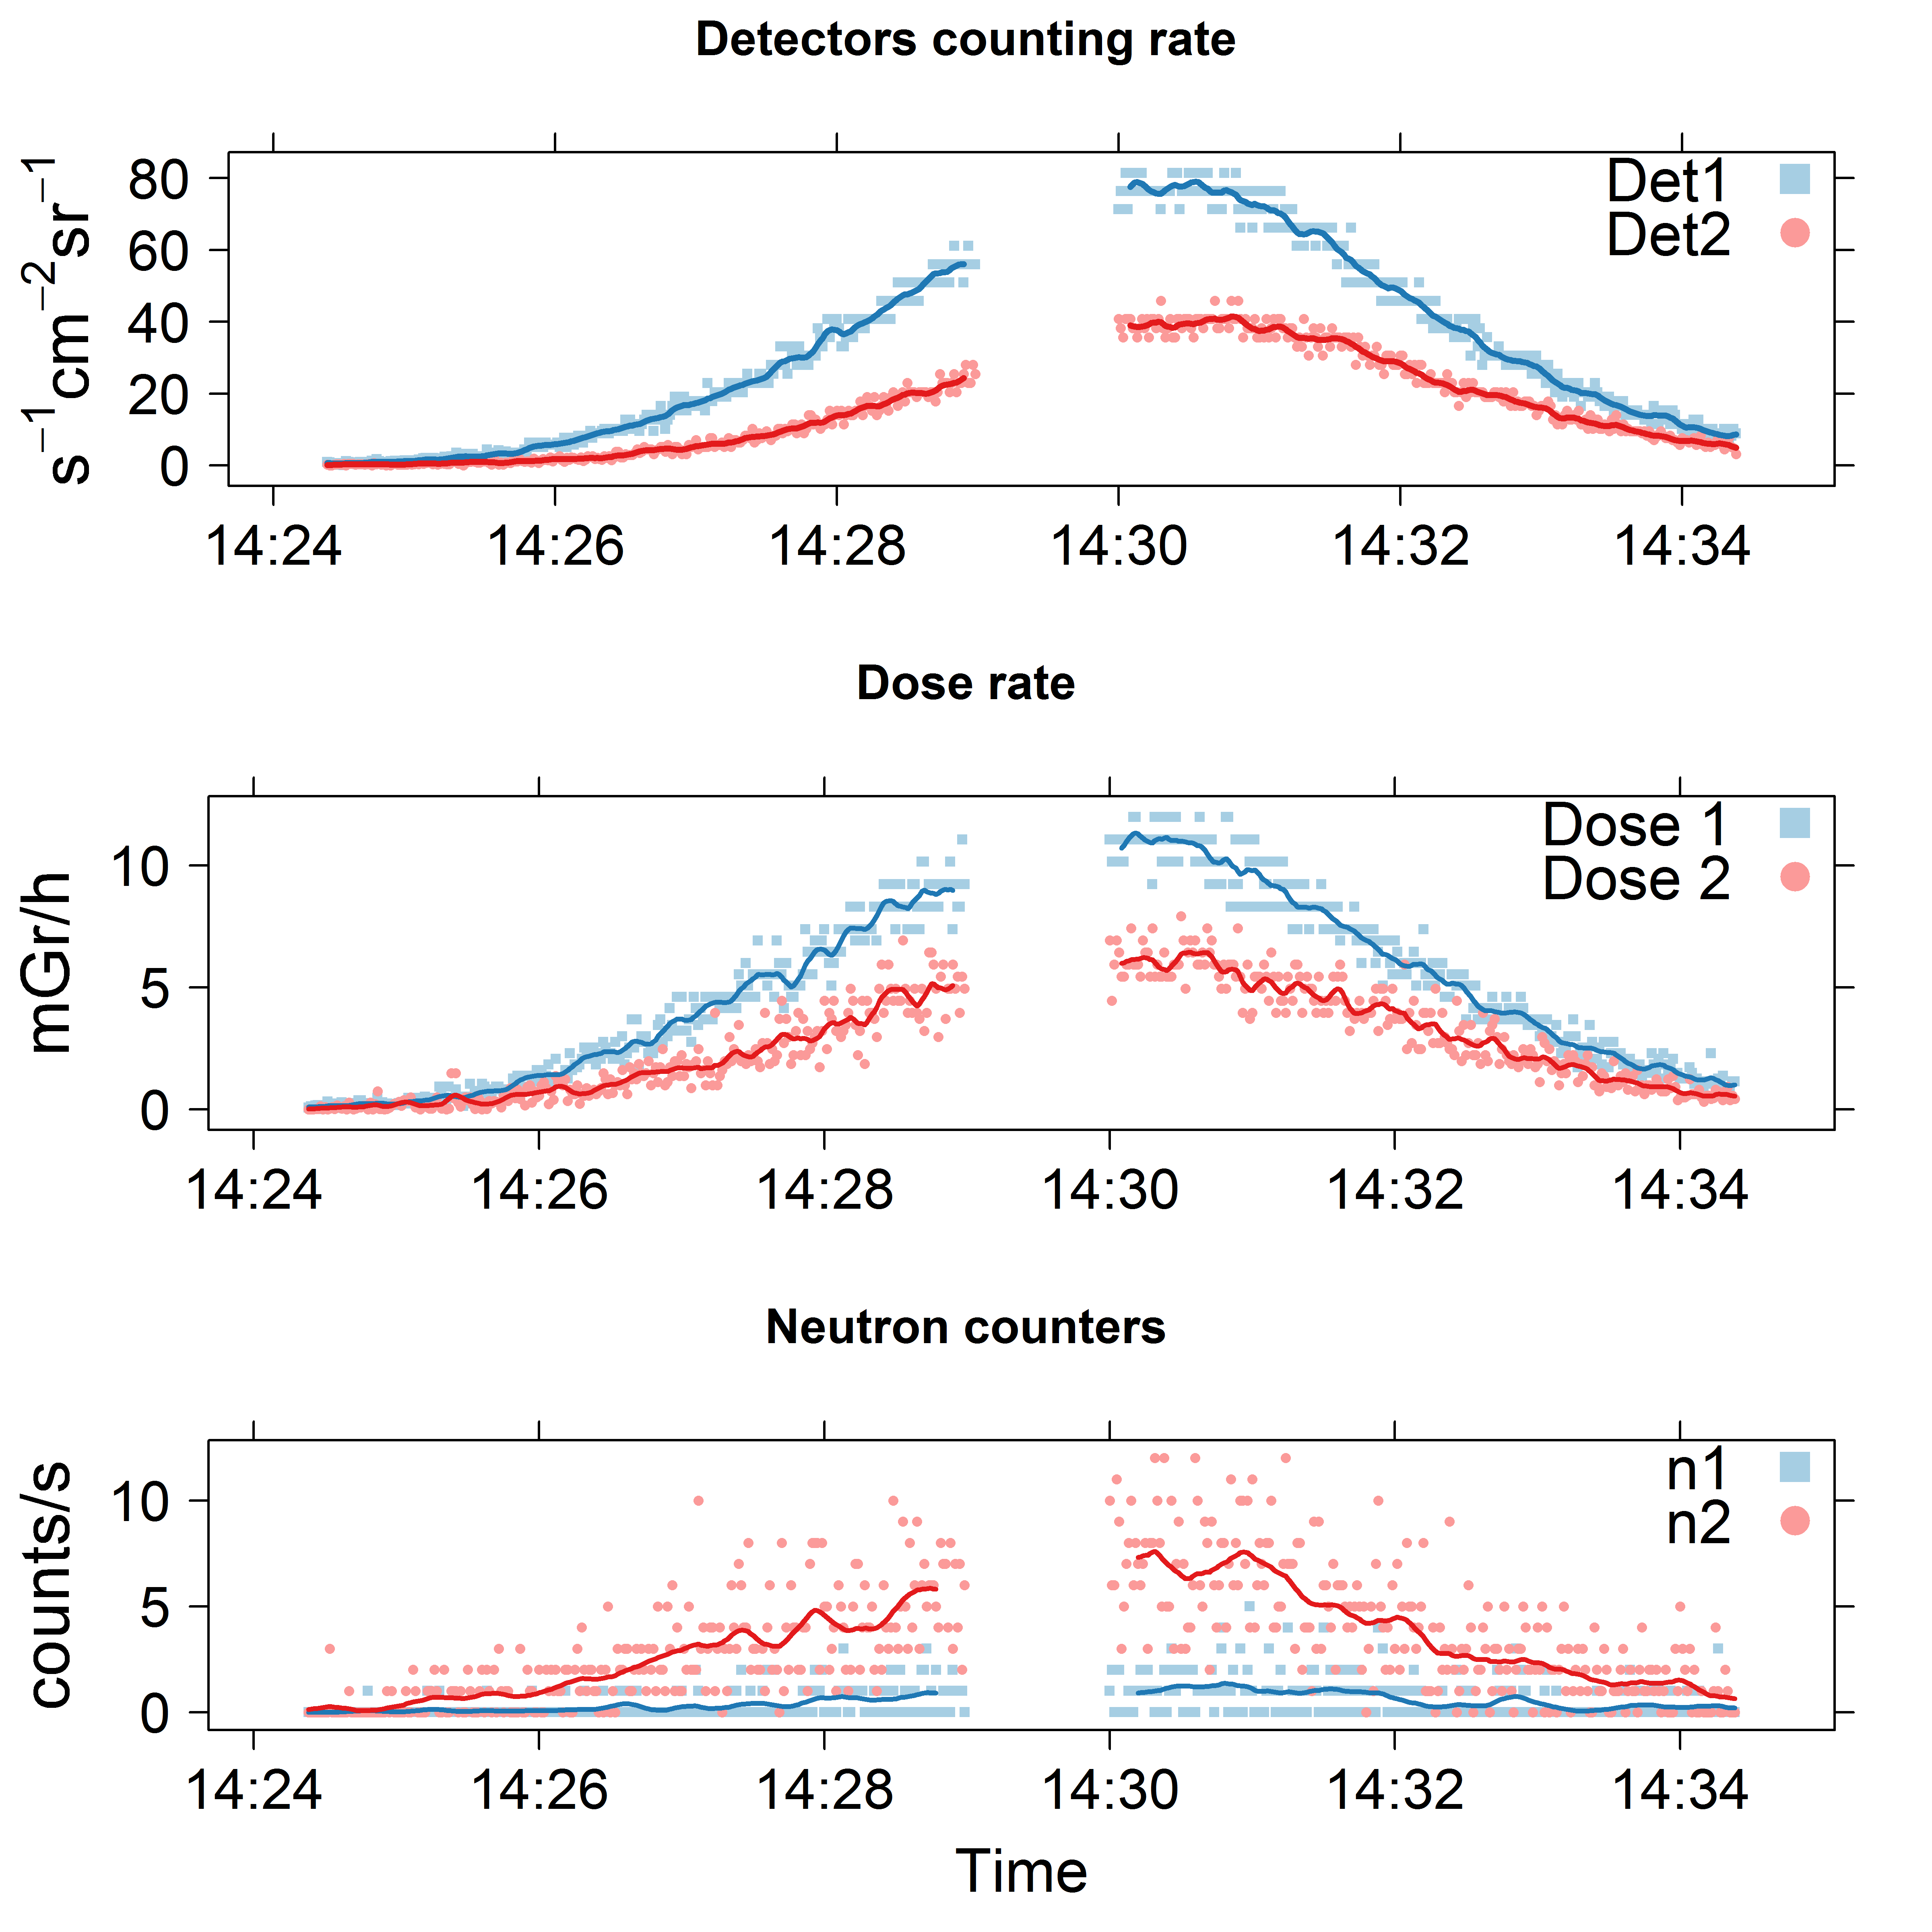
\includegraphics[width=0.7\linewidth]{images/results/depron_sec_log_new08-29-1614-24-23}
	\caption{Временные серии скоростей счета и мошьности дозы при пересечении внутреннего радиационного пояса}	\label{fig:depronseclognew08-29-1614-24-23}
\end{figure}


\section{Распределения мощности дозы в авроральных областях}
Приполярные области отличаются высокой вариабельностью потоков частиц и соответственно доз. В основном повышенные потоки регистрируются в первом полупроводниковом детекторе, что говорит о невысоких энергиях частиц в этих потоках.

\begin{figure}[h]
	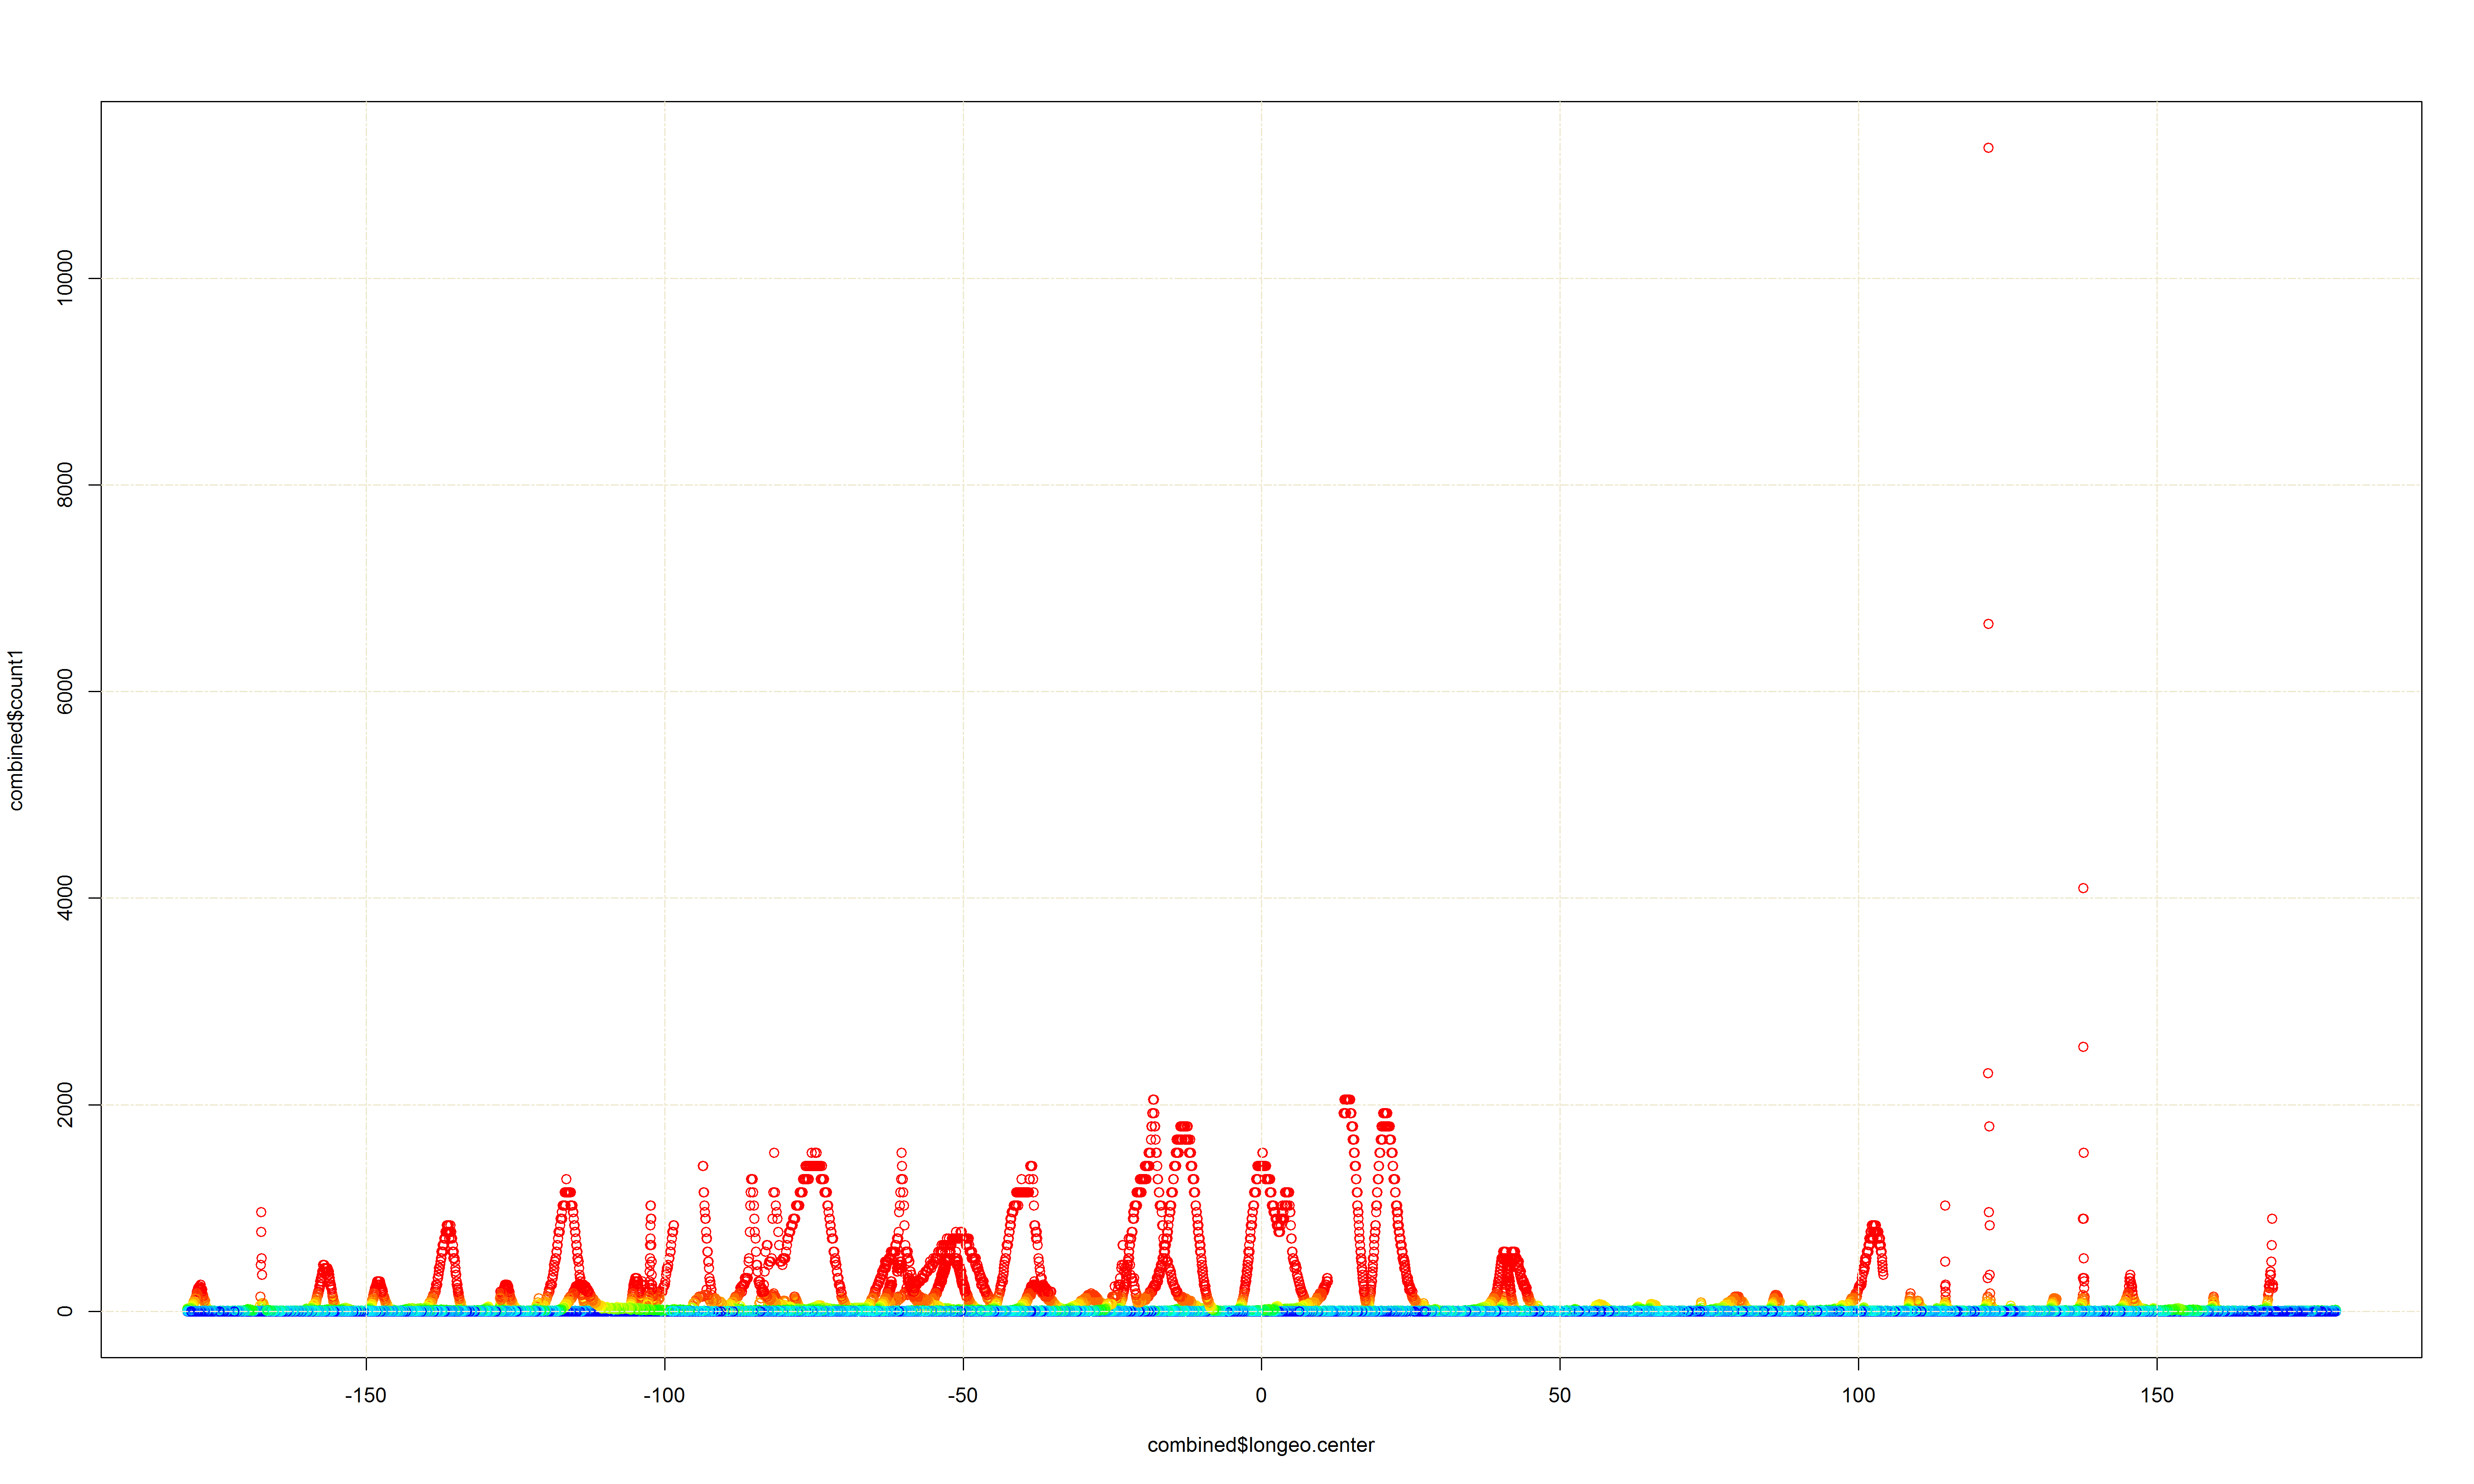
\includegraphics[width=0.8\linewidth]{images/Flash/depron_lat_map_148}
	\caption{Географическое распределение потоков заряженных частиц в первом полупроводниковом детекторе}
	\label{fig:depronlatmap148}
\end{figure}
Рассмотреть зависимости дозы в L-B координатах разделив при этом утреннее в вечернее местное магнитное время (MLT) о наличии магнитной бури следить по индексам A(e) A(l), причем по мнению Антоновой стоит выбрать спокойный период.

Построены зависимости B(t) для L из диапазонов от 4-5, 5-6, 6-7.

\begin{figure}
	\centering
	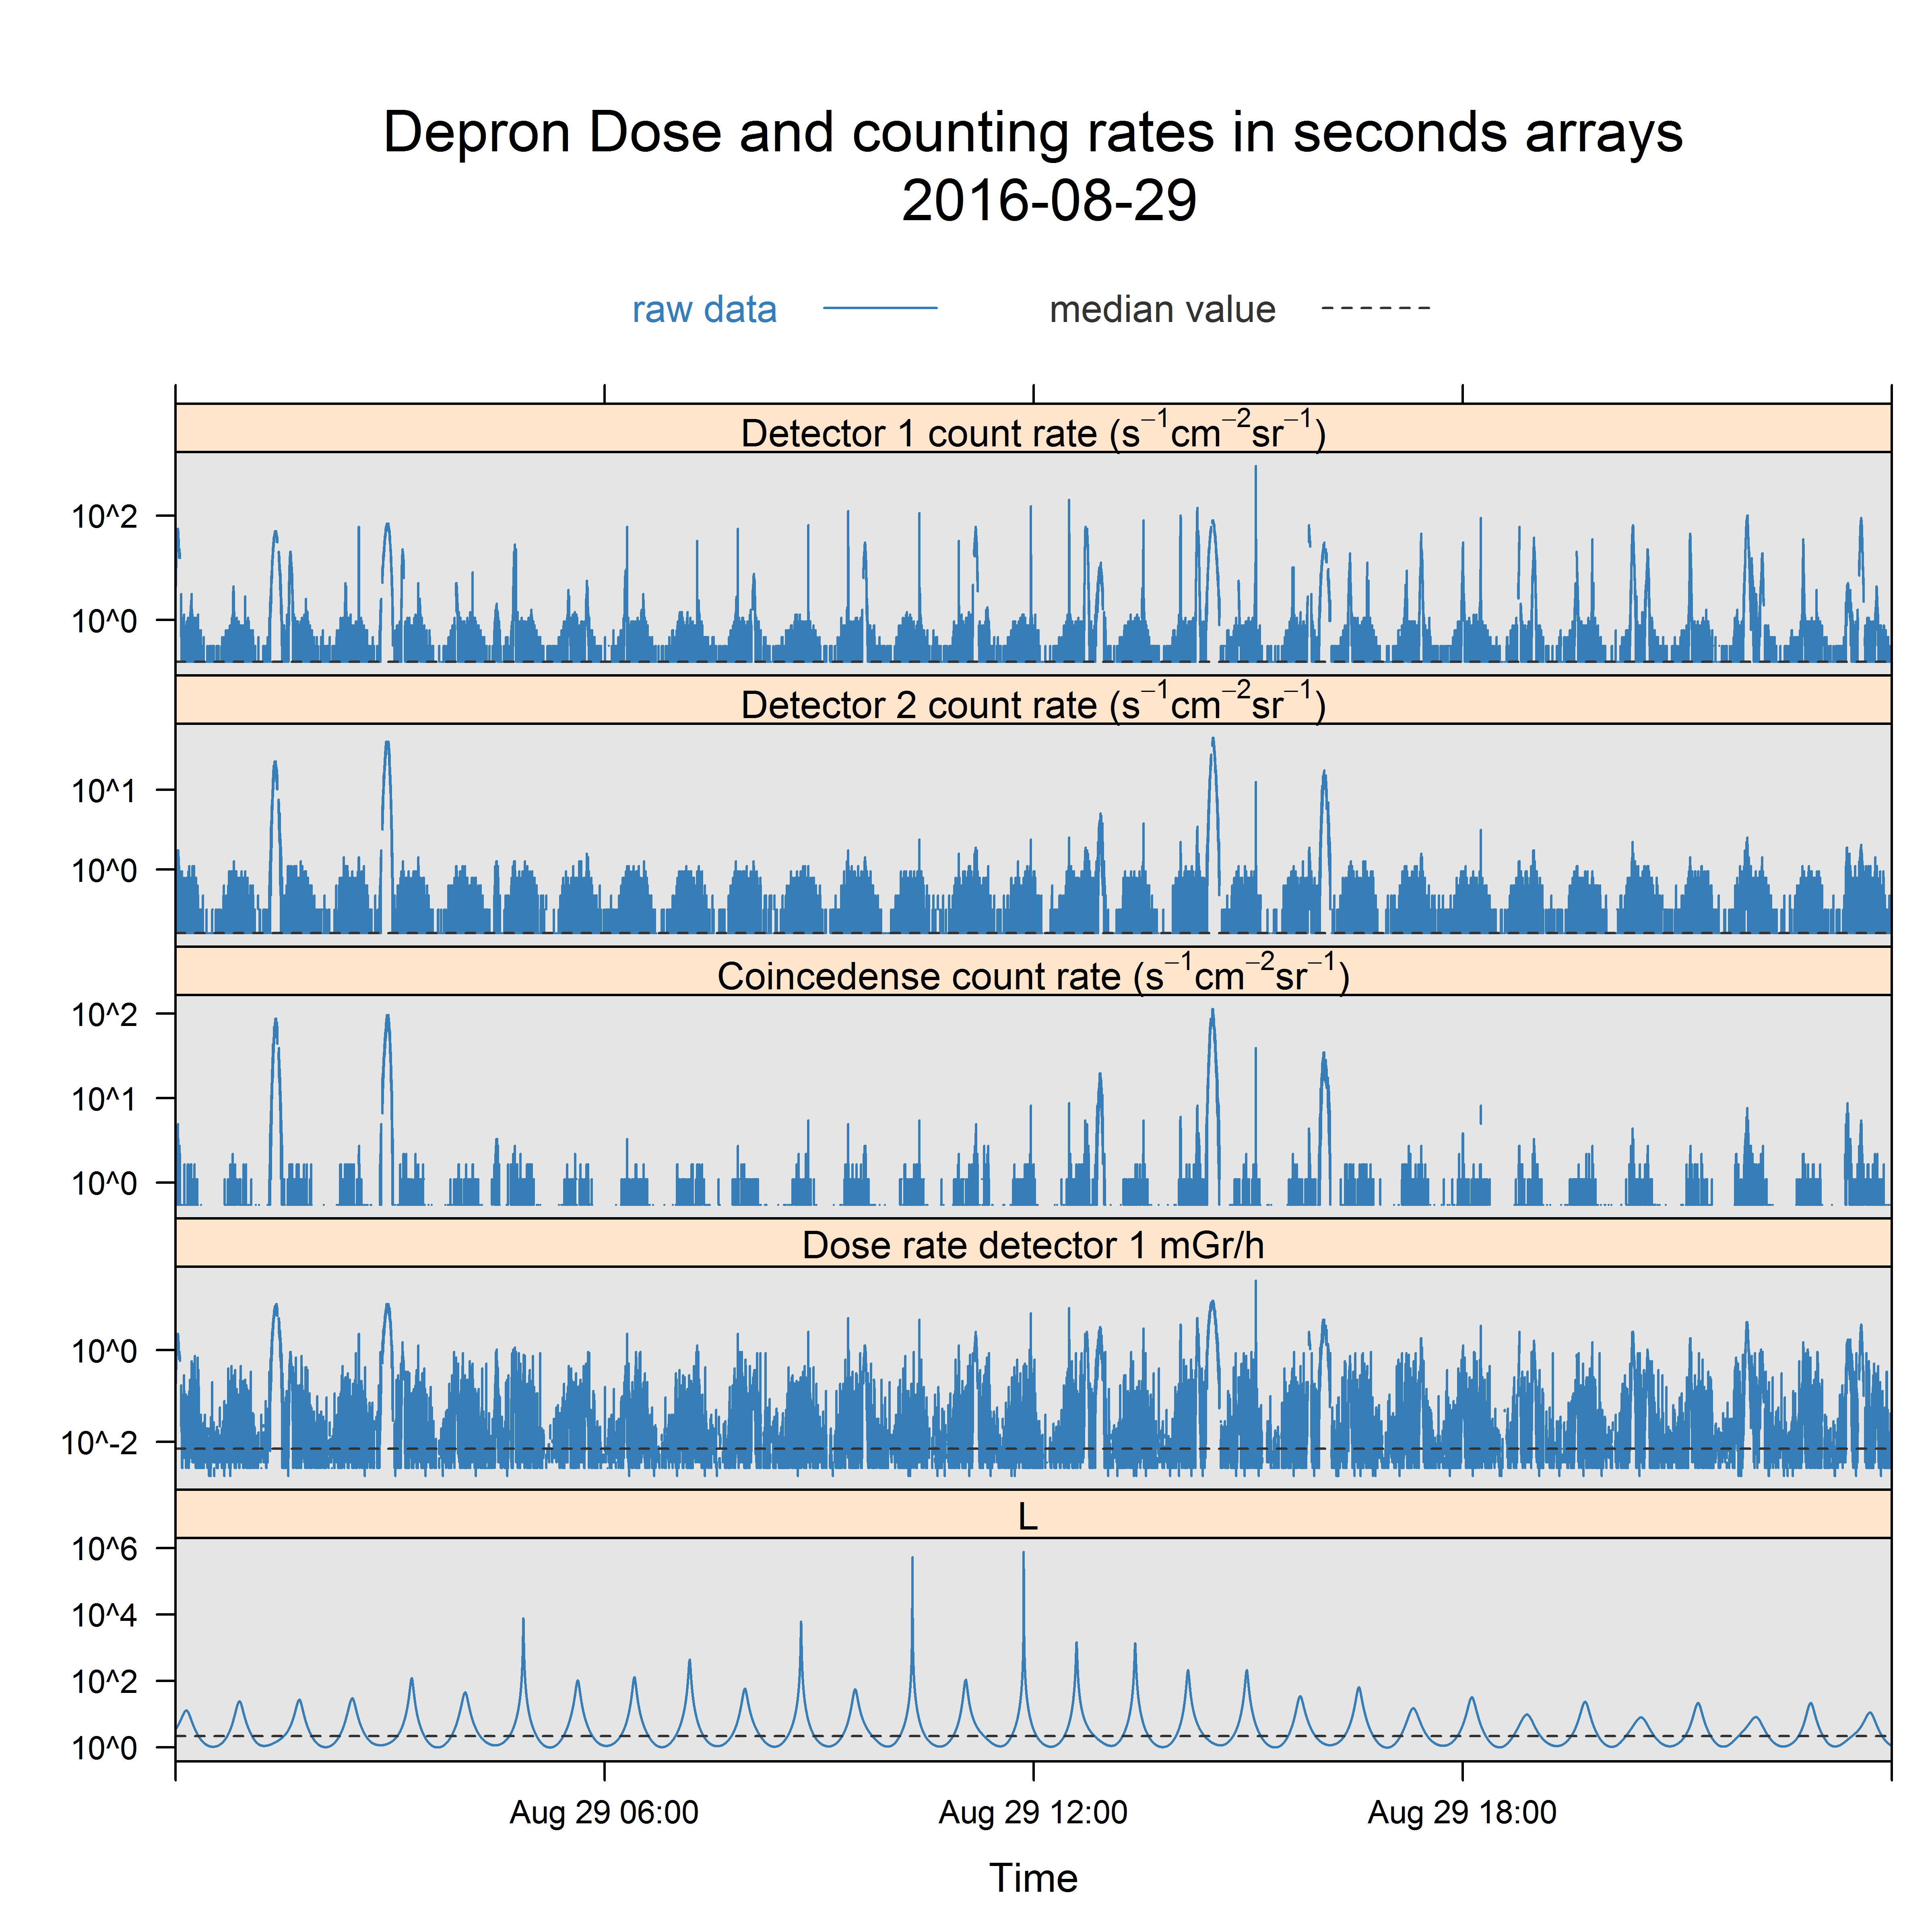
\includegraphics[width=0.7\linewidth]{images/results/depron_sec_log08-29-16}
	\caption{Временные серии в детекторах прибора.}
	\label{fig:depronseclog08-29-16}
\end{figure}
На рисунке \ref{fig:depronseclog08-29-16} показаны 
\begin{figure}
	\centering
	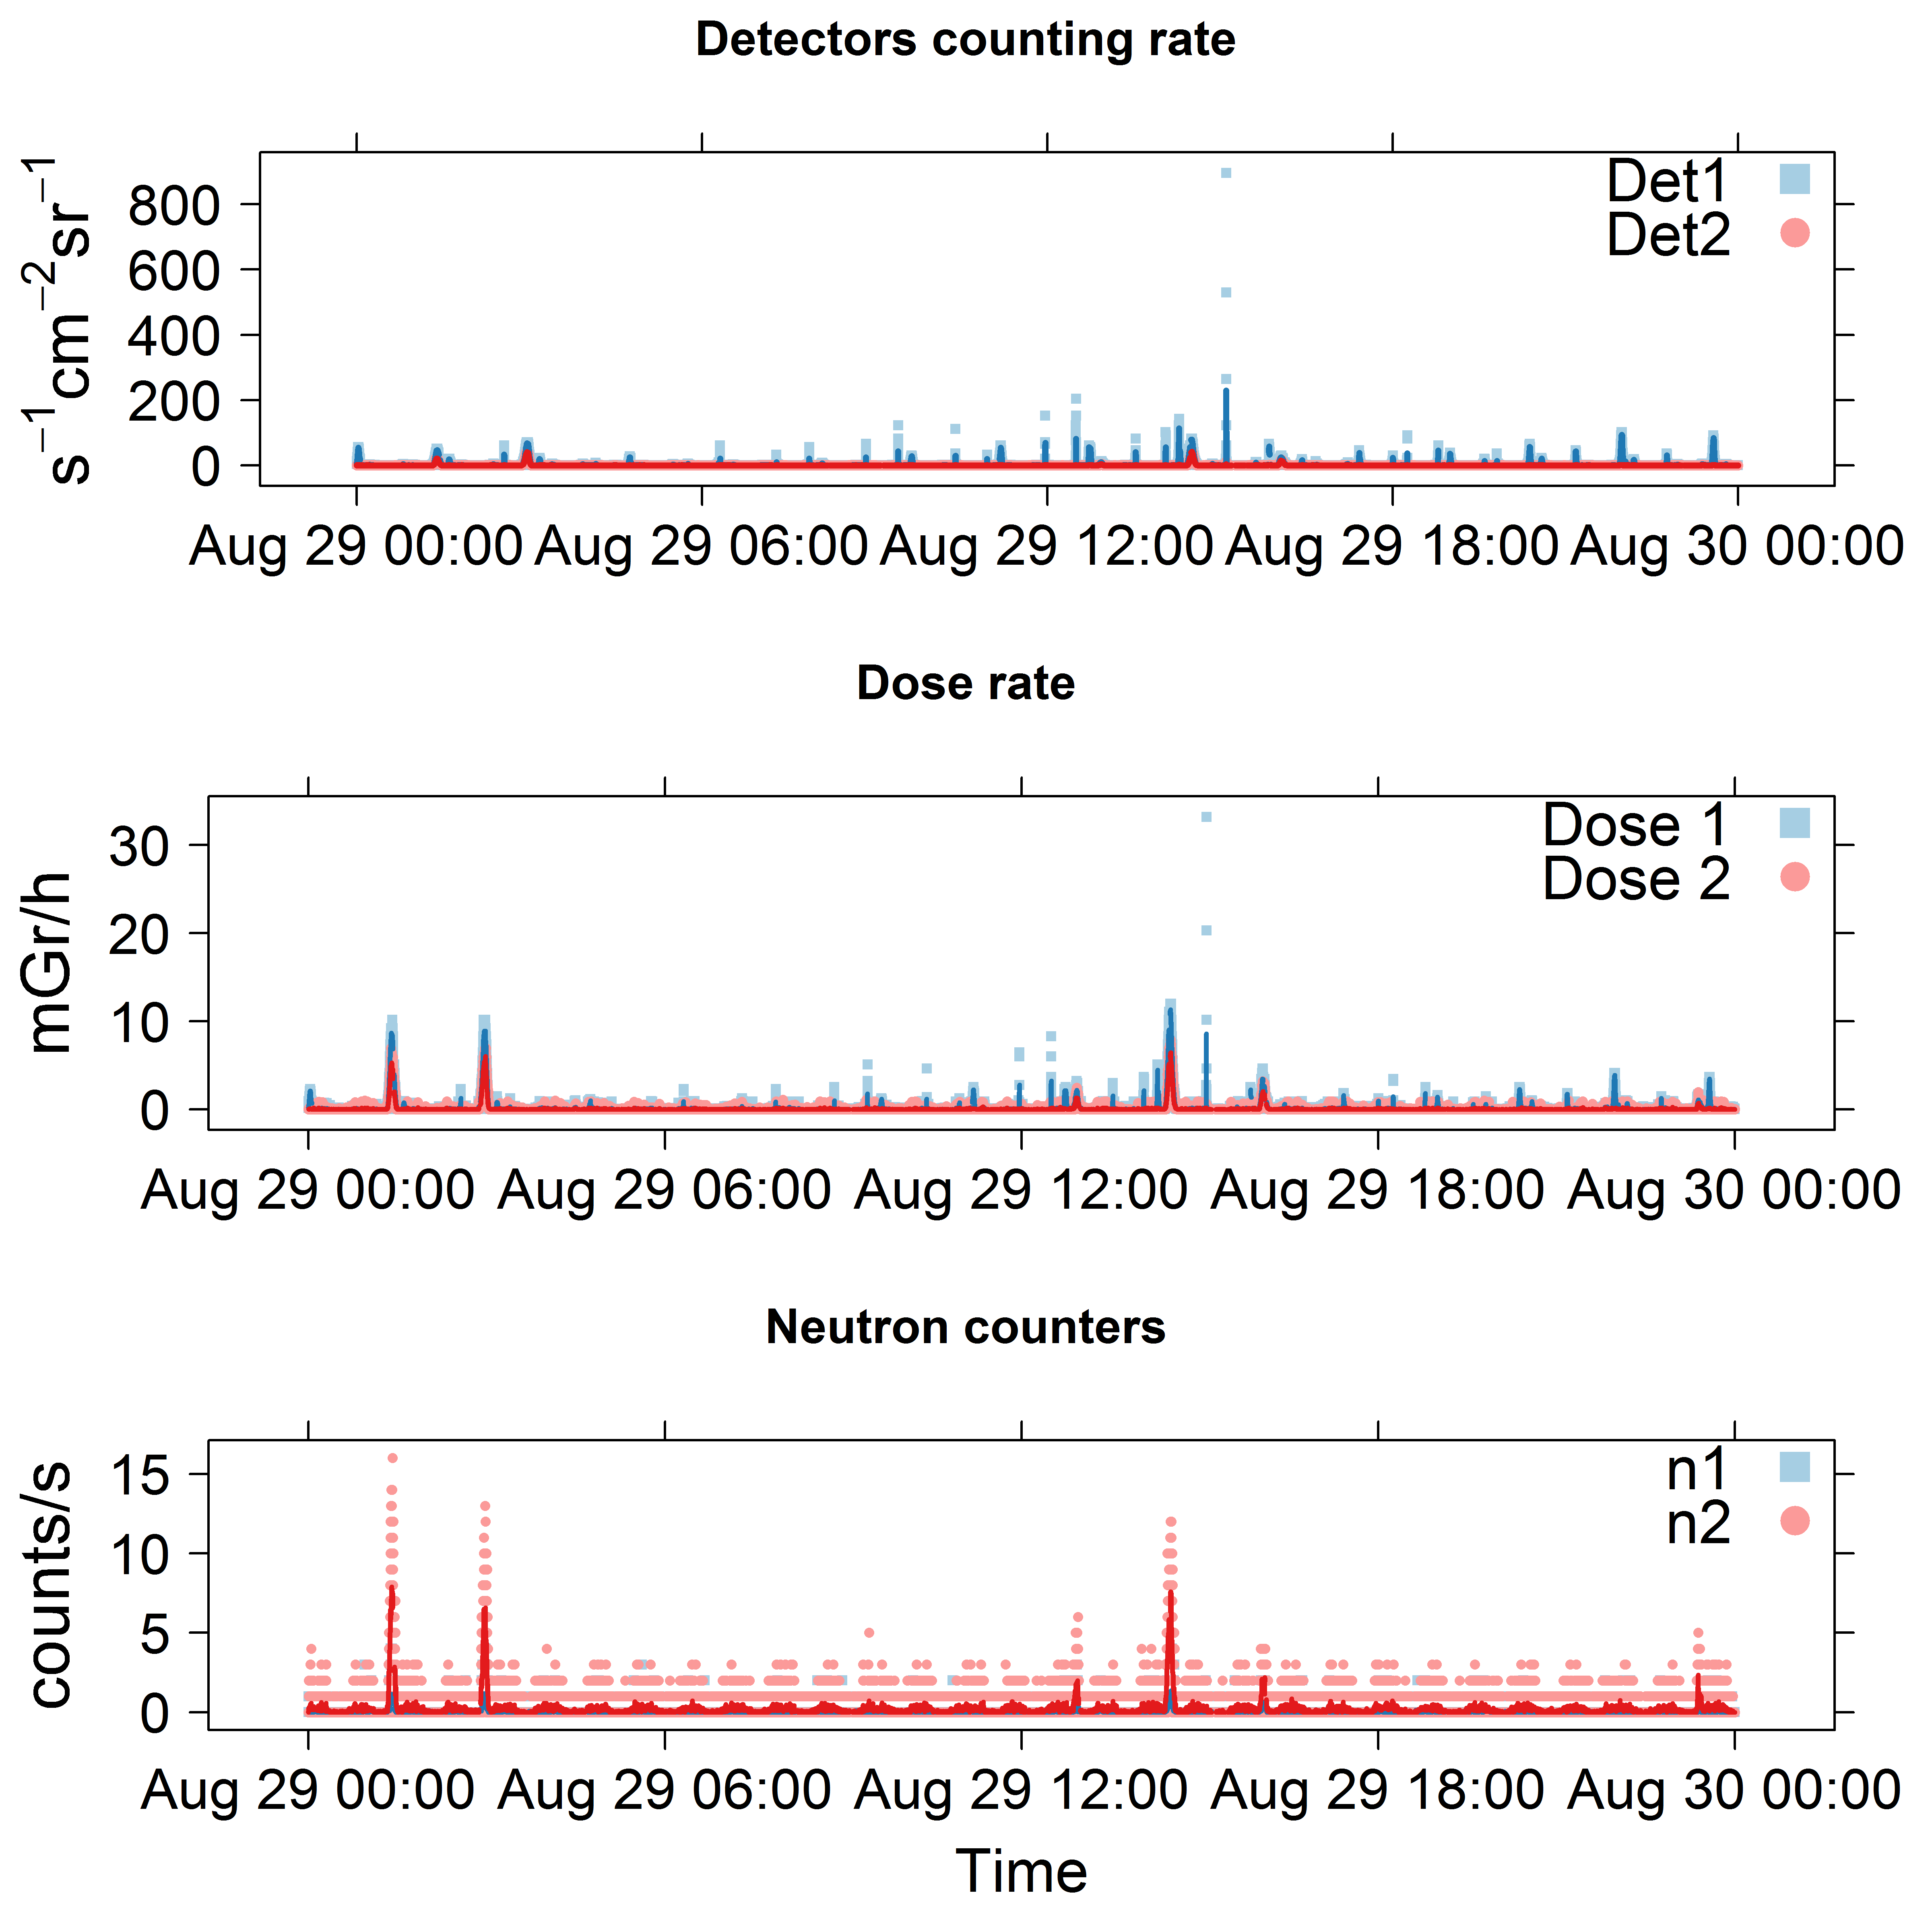
\includegraphics[width=0.7\linewidth]{images/results/depron_sec_log_new08-29-16}
	\caption{}
	\label{fig:depronseclognew08-29-16}
\end{figure}
Счет в детекторах прибора  






\section{Распределение мощности дозы вне радиационных поясов Земли}

\section{Спектры ЛПЭ и распределение мощности эквивалентной дозы}